\section{Objectives}
\label{sec:objectives}
The life-cycle of a Cloud-based IoT application is composed by several states, as illustrated in the Figure \ref{fig:life-cycle}.
% Application Life-cycle
\begin{figure}[h!]
  \centering
  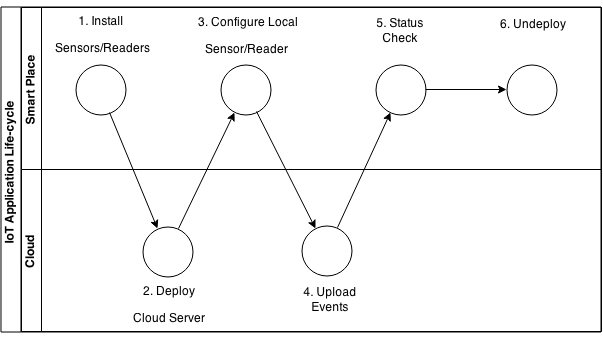
\includegraphics[width=\textwidth]{./images/life-cycle}
  \caption{IoT application life-cycle.}
  \label{fig:life-cycle}
\end{figure}

Thus, the objective of this work is to decrease the complexity of deployment and management of Cloud-based IoT applications in a smart place.
Usually the deployment of such applications is performed by a technician that must manually configure and install the components of the application.
In order to reduce the complexity of this process, the most effective approach is to automate the deployment process of the application. That is achieved
by performing the deployment through Cloud Orchestration tools, that allows to specify the components and the relations between themselves in a high-level
perspective and also provisioning the necessary resources at the Cloud in a effective way. These tools also allows to perform the monitoring of these applications
during its life-cycle as well undeploying them. However, this tools don't solve all our problems. In particular, IoT applications require a software stack that usually
is composed by a database, a web server and the event processing software, in our case the Fosstrak project. But orhcesratation tools normally lacks the integration of
the event processing software with the other components. Thus, to support the integration of such componets these tools must be extend to support the event processing
software.\\

However, managing these applications through a Orchestrator tool requires an elevated technical knowledge. To allow that non-technical users can perform the
managing operations having in perspective the high-level business rules of the smart place, the main objective of this work is to permit that non-technical users
can perform the management of smart spaces only having in mind the business rules of that particular place. To achieve that, these high-level rules must be translated to
a more low-level rules that can be expressed in terms of non-functional requirements that can be used to estimate the resources needed by the application in order
to have an acceptable \textit{QoS}. In the other hand, to allow those non-technical users to monitoring the smart space, these low-level rules must be translated to
a high-level rules that can be expressed in terms of business rules of a given smart space. For instance, if a smart place has a flow of people of 500 persons per day,
that business rule will be translated to non-functional requirements that allows to calculate the amount of storage and bandwidth required to ensure the \textit{QoS}
of the application. Furthermore, by monitoring the service level offered by the Cloud providers it will be possible to determine if the Cloud is overloaded with the
amount of data generated by the smart space or not.
